% ============================================================================
% DESIGN 1 — "THE JOURNAL"
% A reusable, single-file LaTeX report template styled like a premium
% computational-neuroscience journal (Nature Neuroscience / eLife / Neuron).
%
% Compile with:  latexmk -pdf -interaction=nonstopmode report.tex
%
% HOW TO USE THIS TEMPLATE
%   * Everything above the "CONTENT" banner is design/config. Edit the macros
%     in the "AUTHOR-EDITABLE FRONT MATTER" block (title, authors, etc.).
%   * Everything below the "CONTENT" banner is the manuscript body. Swap in
%     your own prose, equations, table rows, figures, and references there.
% ============================================================================

\documentclass[10pt,twocolumn]{article}

% ======================= STYLE / PREAMBLE ===================================
% All design decisions live in this region: packages, fonts, colors, section
% formatting, floats, and custom commands. An author swapping content should
% not need to touch anything here.
% ----------------------------------------------------------------------------

% ---- Page geometry: tight, professional two-column margins -----------------
\usepackage[letterpaper,margin=0.85in,columnsep=0.28in]{geometry}

% ---- Fonts: Cochineal serif for body + math; Biolinum sans for headings ----
\usepackage[T1]{fontenc}
\usepackage[proportional,scaled=0.96]{cochineal} % refined serif, text figures
\usepackage[cochineal]{newtxmath}                  % matching math
\usepackage{biolinum}                              % crisp sans for headings
\usepackage[scaled=0.85]{beramono}                 % compact mono for listings
\usepackage{microtype}                             % refined spacing/protrusion

% ---- Color: exactly one accent (deep teal) --------------------------------
\usepackage[dvipsnames]{xcolor}
\definecolor{accent}{HTML}{0E5C63}   % the single sophisticated accent
\definecolor{rulegray}{HTML}{B9BDC0} % neutral hairlines only

% ---- Core layout / typesetting packages ------------------------------------
\usepackage{titlesec}    % small-caps headings with a colored keyline
\usepackage{tcolorbox}   % full-width tinted abstract box
\tcbuselibrary{skins}    % enables enhanced skin / borderline rules
\usepackage{enumitem}
\usepackage{booktabs}    % clean journal table rules
\usepackage{caption}     % accent figure/table labels
\usepackage{fancyhdr}    % running header with a thin rule
\usepackage{listings}    % code listing
\usepackage{amsmath}
\usepackage{tikz}        % figure placeholder schematic
\usepackage[colorlinks=true,allcolors=accent]{hyperref}

% ---- Running header: short title (left) / page number (right) --------------
\pagestyle{fancy}
\fancyhf{}
\renewcommand{\headrulewidth}{0.4pt}
\renewcommand{\headrule}{\hbox to\headwidth{\color{rulegray}\leaders\hrule height \headrulewidth\hfill}}
\fancyhead[L]{\footnotesize\scshape\thetitleshort}
\fancyhead[R]{\footnotesize\thepage}

% ---- Section headings: sans small caps + accent number + accent keyline ----
\titleformat{\section}
  {\normalfont\sffamily\bfseries\large\scshape}
  {\color{accent}\thesection}{0.6em}{}
  [\vspace{2pt}{\color{accent}\titlerule[0.9pt]}]
\titleformat{\subsection}
  {\normalfont\sffamily\bfseries\normalsize}
  {\color{accent}\thesubsection}{0.5em}{}
\titlespacing*{\section}{0pt}{1.4ex plus .3ex}{0.8ex}
\titlespacing*{\subsection}{0pt}{1.1ex plus .2ex}{0.5ex}

% ---- Captions: small bold accent label, smaller caption text ---------------
\captionsetup{
  font=small,
  labelfont={bf,color=accent},
  labelsep=period,
  justification=justified,
  singlelinecheck=false
}

% ---- Code listing style (monochrome, journal-restrained) -------------------
\lstdefinestyle{journal}{
  basicstyle=\ttfamily\scriptsize,
  keywordstyle=\color{accent}\bfseries,
  commentstyle=\itshape\color{rulegray},
  numberstyle=\tiny\color{rulegray},
  language=Python,
  showstringspaces=false,
  breaklines=true,
  columns=fullflexible,
  frame=leftline,
  framesep=6pt,
  rulecolor=\color{accent},
  xleftmargin=8pt,
  aboveskip=1ex,belowskip=0.5ex,
}
\lstset{style=journal}

% ---- Custom command: full-width abstract box (spans both columns) ----------
\newcommand{\abstractbox}[1]{%
  \begin{tcolorbox}[
      enhanced, sharp corners, boxrule=0pt, frame hidden,
      colback=accent!5, borderline west={2pt}{0pt}{accent},
      left=10pt,right=10pt,top=8pt,bottom=8pt,
      before skip=4pt, after skip=10pt]
    \small
    {\sffamily\bfseries\scshape\color{accent}Abstract\quad}#1
  \end{tcolorbox}%
}

% ======================= AUTHOR-EDITABLE FRONT MATTER =======================
% Swap these macros for the real manuscript metadata.
% ----------------------------------------------------------------------------
\newcommand{\thetitlefull}{Decision Making in Low-Rank Recurrent Neural Networks}
\newcommand{\thetitleshort}{Decision Making in Low-Rank RNNs} % running head
\newcommand{\theauthors}{Arjun Puri \quad Samuel Delsol \quad Sebastian Valero Dorado}
\newcommand{\theaffiliation}{Department of Neuroscience, [Institution].\quad
  Correspondence: \href{mailto:arjunpur2@gmail.com}{arjunpur2@gmail.com}}
\newcommand{\thedate}{July 2026}

% ============================================================================
% ============================  CONTENT  =====================================
% Everything below is the manuscript. Replace prose, equations, table rows,
% and references with your own; the styling above will carry through.
% ============================================================================
\begin{document}

% ---- Full-width title block (single column across the page) ----------------
\twocolumn[
  \begin{@twocolumnfalse}
    \begingroup\centering
      {\color{accent}\rule{\textwidth}{1.1pt}}\par\vspace{0.6em}
      {\sffamily\bfseries\LARGE \thetitlefull\par}\vspace{0.7em}
      {\scshape\large \theauthors\par}\vspace{0.4em}
      {\footnotesize \theaffiliation\par}\vspace{0.2em}
      {\footnotesize \thedate\par}\vspace{0.5em}
      {\color{accent}\rule{\textwidth}{0.4pt}}\par
    \endgroup
    \vspace{0.4em}
    % ---- Full-width abstract spanning both columns ----
    \abstractbox{Abstract text goes here. Summarise the motivation, approach,
      and main findings in a short paragraph.}
    \vspace{0.6em}
  \end{@twocolumnfalse}
]

% ---------------------------------------------------------------------------
\section{Introduction}

Introductory paragraph. State the problem, prior work, and the question this
report addresses.

A second introductory paragraph expanding on context and outlining the
structure of the remainder of the report.

% ---------------------------------------------------------------------------
\section{Results}

Overview of the main results.

\subsection{First result}

Description of the first result. Replace with findings, figures, and
interpretation.

\subsection{Second result}

Description of the second result. Replace with findings, figures, and
interpretation.

% ---- Figure placeholder (in-document TikZ schematic; no external asset) ----
\begin{figure}[t]
  \centering
  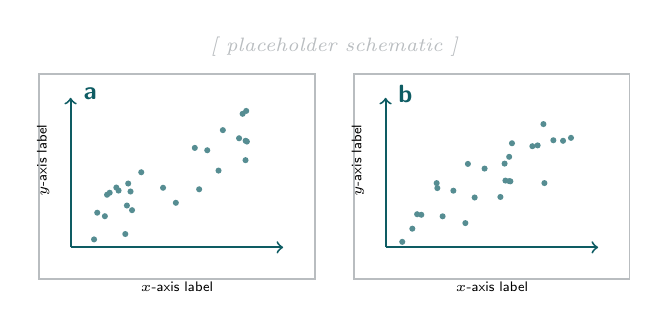
\begin{tikzpicture}
    % Panel (a)
    \begin{scope}
      \draw[rulegray,line width=0.6pt] (0,0) rectangle (3.5,2.6);
      \draw[->,accent,line width=0.7pt] (0.4,0.4)--(3.1,0.4);
      \draw[->,accent,line width=0.7pt] (0.4,0.4)--(0.4,2.3);
      \foreach \i in {1,...,26}{
        \pgfmathsetmacro{\x}{0.6+2.2*rnd}
        \pgfmathsetmacro{\y}{0.6+0.6*(\x-0.6)+0.35*rand}
        \fill[accent!70] (\x,\y) circle (1.1pt);
      }
      \node[font=\tiny\sffamily] at (1.75,-0.1) {$x$-axis label};
      \node[font=\tiny\sffamily,rotate=90] at (0.05,1.5) {$y$-axis label};
      \node[font=\sffamily\bfseries\small,accent] at (0.65,2.35) {a};
    \end{scope}
    % Panel (b)
    \begin{scope}[xshift=4.0cm]
      \draw[rulegray,line width=0.6pt] (0,0) rectangle (3.5,2.6);
      \draw[->,accent,line width=0.7pt] (0.4,0.4)--(3.1,0.4);
      \draw[->,accent,line width=0.7pt] (0.4,0.4)--(0.4,2.3);
      \foreach \i in {1,...,26}{
        \pgfmathsetmacro{\x}{0.6+2.2*rnd}
        \pgfmathsetmacro{\y}{0.6+0.55*(\x-0.6)+0.4*rand}
        \fill[accent!70] (\x,\y) circle (1.1pt);
      }
      \node[font=\tiny\sffamily] at (1.75,-0.1) {$x$-axis label};
      \node[font=\tiny\sffamily,rotate=90] at (0.05,1.5) {$y$-axis label};
      \node[font=\sffamily\bfseries\small,accent] at (0.65,2.35) {b};
    \end{scope}
    \node[font=\scriptsize\itshape,rulegray] at (3.75,2.95)
      {[ placeholder schematic ]};
  \end{tikzpicture}
  \caption{Figure caption. Describe panels (a) and (b) and what the reader
    should take away.}
  \label{fig:placeholder}
\end{figure}

% ---------------------------------------------------------------------------
\section{Methods}

\subsection{Model}

Describe the model. Example equations are shown below; replace with your own.

\begin{equation}
  \tau\,\frac{dx_i}{dt}
  = -x_i + \sum_{j=1}^{N} J_{ij}\,\phi(x_j)
  + \sum_{s=1}^{N_{\mathrm{in}}} I_i^{(s)}\,u_s(t)
\end{equation}

\begin{equation}
  J_{ij} = \frac{1}{N}\sum_{r=1}^{R} m_i^{(r)}\,n_j^{(r)}
\end{equation}

\subsection{Training}

Describe the training procedure. Hyperparameters are summarised in
Table~\ref{tab:hyper}. An example forward pass is given in the listing below.

\begin{equation}
  z(t) = \frac{1}{N}\sum_{i=1}^{N} w_i\,\phi(x_i)
\end{equation}

% ---- Table 1: hyperparameters (booktabs) ----
\begin{table}[t]
  \centering
  \caption{Training hyperparameters.}
  \label{tab:hyper}
  \small
  \begin{tabular}{@{}ll@{}}
    \toprule
    \textbf{Parameter} & \textbf{Value} \\
    \midrule
    Parameter A        & value \\
    Parameter B        & value \\
    Parameter C        & value \\
    \bottomrule
  \end{tabular}
\end{table}

% ---- Code listing ----
\begin{lstlisting}[caption={Example code listing.},captionpos=b]
def forward(self, u):
    # placeholder
    return z
\end{lstlisting}

% ---------------------------------------------------------------------------
\section{Discussion}

Discuss the implications of the results, limitations, and next steps.

% ---------------------------------------------------------------------------
\section*{References}
\begin{enumerate}[label={[\arabic*]},leftmargin=*,itemsep=2pt,font=\bfseries]
  \item Author, A., and Author, B. (Year). Title of the paper. \textit{Journal}, volume, pages.
  \item Author, C., et al.\ (Year). Title of the paper. \textit{Journal}, volume, pages.
\end{enumerate}

\end{document}
